
\chapter{Opis projektnog zadatka}

\normalfont{
	Cilj ovog projekta je razviti novu personaliziranu platformu u obliku web aplikacije koja će se koristiti za promociju zabavnih događanja u gradu. Za korištenje aplikacije potrebno je registrirati se kao organizator ili posjetitelj.
	Organizatori zabavnih događanja postavljaju najave za događanja koja organiziraju (koncerti, događanje u klubovima, kazališne predstave, ...) i obvezni su plaćati mjesečnu članarinu putem PayPala ili kreditne kartice, dok zainteresirani posjetitelji besplatno koriste aplikaciju te mogu najaviti svoj dolazak na neki događaj i pisati recenzije. Organizatori imaju svoje javne profile na kojima se nalaze osnovni podaci:}

\begin{packed_item}
	\item \normalfont{naziv}
	\item \normalfont{adresa}
	\item \normalfont{poveznice na vlastite web ili Facebook stranice}
	\item \normalfont{popis svih događanja koja su oglašena putem aplikacije u zadnje 2 godine}
\end{packed_item}

\normalfont\noindent{Za svako događanje dostupni su detalji: }

\begin{packed_item}
	\item \normalfont{naziv}
	\item \normalfont{vrsta}
	\item \normalfont{lokacija}
	\item \normalfont{vrijeme početka i trajanje}
	\item \normalfont{foto/video galerija}
	\item \normalfont{popis svih recenzija vezanih uz to događanje}
\end{packed_item}
\normalfont {(Podatke o događanju, fotografije i video unose organizatori.)}

\normalfont\noindent {Posjetitelji u aplikaciji mogu vidjeti popis aktualnih događanja u odabranom vremenskom razdoblju (24 sata, 7 dana, 30 dana) te mogu za svako događanje izraziti interes („sigurno dolazim“, „možda dolazim“, „ne dolazim“) koji se može promijeniti ukoliko se predomisle. Na taj način organizatori vide kolika je zainteresiranost za pojedino događanje, a pošto je broj zainteresiranih javno vodljiv uz događanje na profilu organizatora, posjetitelji mogu vidjeti koliko će ljudi otprilike prisustvovati događanju. Posjetitelji također mogu pisati recenzije za događanja koja su završila u proteklih 48 sati te mogu namjestiti postavke da im aplikacija automatski šalje obavijesti o najnovijim događanjima prema zadanim kriterijima: vrsta događanja i područje.}

\normalfont {U sustavu osim organizatora i posjetitelja postoje i administratori koji postavljaju cijenu članstva te upravljaju korisnicima. Ukoliko organizator nije podmirio svoju mjesečnu članarinu ne može pristupiti svom računu te s obzirom na to nije u mogućnosti vidjeti ili mijenjati već postojeća događanja niti kreirati nova. Prilikom prijave na svoj račun jedino što organizator može napraviti je podmiriti svoje dugove.}

\begin{figure}[h]
	\centering
	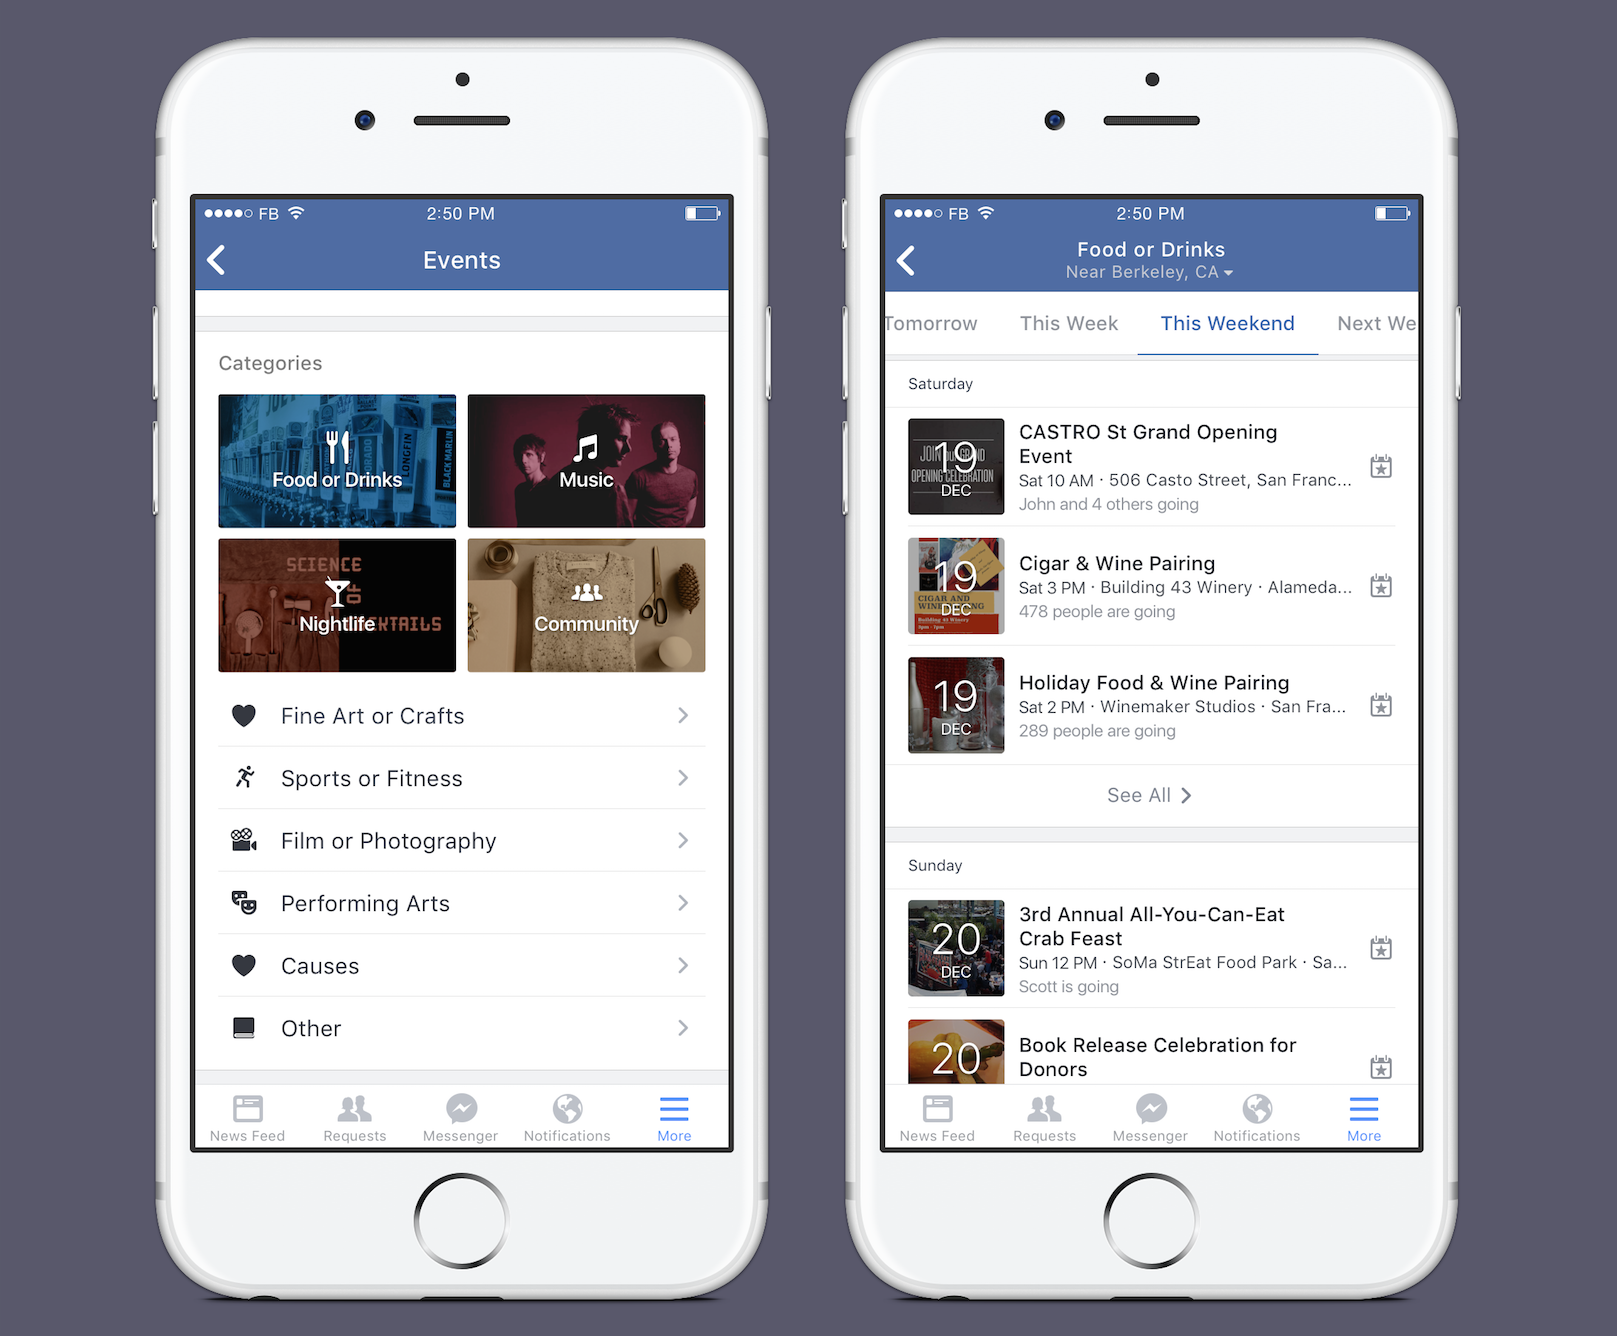
\includegraphics[width=\linewidth]{slike/facebook_events.PNG}
	\caption{Facebook događaji}
	\label{fig:primjer}
\end{figure}

\normalfont{Slično postojeće rješenje su \textit{Facebook događaji} gdje se mogu vidjeti najave za razna zabavna događanja, izraziti interes za njih, pisati recenzije i vidjeti fotografije. Razlika je u tome što ne postoje organizatori i posjetitelji, već se svi jednako i besplatno registriraju. Pošto nema razlike među korisnicima svatko može napraviti najavu za događanje koja nam daje kratki opis događanja i informacije o lokaciji, njegovom početku i trajanju, broju ljudi koji su zainteresirani za njega, itd. Pošto je ovo slično rješenje dio društvene mreže \textit{Facebook} postoji još dodatnih mogućnosti kao što su: slanje poziva za neko događanje prijateljima, komentiranje tuđeg interesa za neko događanje, i slično.
Društvenu mrežu \textit{Facebook} koristi jako puno ljudi koji pripadaju raznim skupinama, a svi koji ga koriste služe se i njegovom opcijom za organizaciju događanja (\textit{Facebook događaji}). Neki ga koriste isključivo zbog toga što na jednom mjestu mogu imati organizirani pregled događanja za koja su zainteresirani. Stoga smatram da bi i ova naša platforma bila popularna unutar više različitih skupina ljudi.}

\normalfont{Platforma koju smo napravili jedna je od mogućih verzija koja zadovoljava uvijete zadane projektnim zadatkom, no to ne znači da se nije moguća nadogradnja. Neki od mogućih dodataka su: ocjene od 1 do 5 kojima bi posjetitelji mogli ocijeniti događanje bez pisanja recenzija, mogućnost kupovine ulaznica i reklamnih materijala putem aplikacije, forum za korisnike na kojem bi mogli davati ideje kako unaprijediti aplikaciju, ...}

\eject
